
\documentclass[11pt,a4paper]{article}
\usepackage{amsmath}
\usepackage{amsfonts}
\usepackage{graphics}
\usepackage{supertabular}
\usepackage{grffile}
\usepackage{color}
\usepackage{tikz}

\title{\bf Moment based tool for genetic diversity simulations and demographic inference.} 
\author{Julien Jouganous, Simon Gravel}
\newcommand\p[2]{\frac{\partial #1}{\partial #2}}
\newcommand\pd[2]{\frac{\partial^2 #1}{\partial #2^2}}
\newcommand\pn[3]{\frac{\partial^#1 #2}{\partial #3^#1}}
\newcommand\dadi{\partial a \partial i} 

\bibliographystyle{plain} 

\begin{document}

\maketitle

\section*{abstract}

\section{Introduction}
Inferring populations histories is a critical issue in modern sciences. Applied to the human species, it might help us understand where we come from, from a geographical and also an evolutionary point of view.
A first way to learn about populations histories is to look for archeological evidences. Carbon dating technics, introduced in the 1950s by Willard Franck Libby \cite{libby1949}, made it possible to date quite accurately some of these relatively recent evidences of human activity \cite{valladas2001}. Other comparable technics are better adapted to date older events \cite{walter1994}.

In recent years, massive genome sequencing experiments have generated large amounts of data that can be used to confirm or complement archeological theories. Indeed, demographic events as migrations, populations splits or selective pressure have repercussions on genetic diversity among populations. Reversely, quantifying and studying this diversity may help reconstruct the population history. In this context, demographic models can be compared to genetic data using some specific statistics as the allele frequency spectrum (AFS). To this aim, we need to be able to model and simulate these statistics as well as the effects of demographic events and populations histories. Then, we infer the best model and values for the demographic parameters, \textit{i.e.} the most likely knowing the observed data.

There are different ways to model the evolution of the AFS. On the one hand, one can use a backward approach, based on coalescence theory \cite{excoffier2011}. If these methods may be appropriate for neutral simulations, they are initially not designed to take into account selective pressures. On the other hand, forward in time tools have been developed. Most of them are based on the diffusion approximation initiated by Fisher and Wright in the 1930' \cite{fisher1930, wright1931} and then extended more recently \cite{crow1970, kimura1964}. In this approach, the evolution of the AFS is described as a continuous process through a partial differential equation. This formalism makes it possible to take into account a wider variety of demographic and evolutionary processes such as selection and dominance. Several simulating tools based on this diffusion approximation have been implemented and distributed to the population genetics community \cite{gutenkunst2009, lukic2012, lukic2011}, among which $\dadi$ is probably one of the most commonly used. In the past few years, these numerical tools have been used in many works and led to significant results from both historical and biological points of view \cite{gutenkunst2009, gravel2011, schmutz2014}. However, these technics generally involve different levels of numerical approximations such as time and frequency space discretization or numerical computation of integrals.Their use is limited to relatively simple data sets, for instance, $\dadi$ cannot handle more than 3 populations at the time. Moreover, the demographic inference needs numerous simulations of the model and the computation time is a critical challenge if we want to calibrate complex models.

In this document/paper, we describe a new efficient tool to simulate genetic diversity based on the diffusion approximation. We use this method to infer populations histories from genetic data.

\section{Method and material}

\subsection{The diffusion approximation}
The diffusion approximation applied to the Wright-Fisher model for a single diploid population with drift, selection and mutations (see \cite{kimura1964} for more details) writes:
\begin{equation}
	\begin{split}
	\p{\phi(x,t)}{t}\simeq &\frac{1}{4 N} \pd{}{x} x(1-x) \phi(x,t) \\&-s \p{}{x} \left(h+(1-2h)x \right)x (1-x) \phi(x,t) \\&+ 2 N u \delta(x-\frac{1}{2 N}).
	\end{split}
	\label{eq:diff}
\end{equation}

This partial differential equation describes the evolution of the density of allele frequencies $\phi(x,t)$ (\textit{i.e.} the expected proportion of derived mutations at frequency $x \in [0, 1]$ in the population and at time $t$). In this equation $N$ is the population size and $s$, $h$ and $u$ are respectively the selection coefficient, the dominance coefficient and the mutation rate.
The first term of the right hand side, $\frac{1}{4 N} \pd{}{x} x(1-x) \phi(x,t)$, describes genetic drift as a diffusion process. Selection is modeled by the transport-like term $-s \p{}{x} \left(h+(1-2h)x \right)x (1-x) \phi(x,t)$ whereas the source term $2 N u \delta(x-\frac{1}{2 N})$ accounts for \textit{de novo} mutations. The expression $\delta(x-\frac{1}{2 N})$ is the Dirac distribution peaked at frequency $\frac{1}{2 N}$. It corresponds to the infinite site model \cite{kimura1969}, assuming that each time a mutation appears it affects a locus previously unaffected. So, in this case, we do not consider back mutations.

The approximation leading to this equation is valid for large effective population size $N >> 1$ and for small values of selection coefficients and migration rates (when dealing with several populations), comparable to the ratio $\frac{1}{N}$. 

The distribution of allele frequencies $\phi(x,t)$ cannot be directly observed in genome sequencing data. However, we can construct the histogram of the occurrences of the variant alleles in a given sample. This histogram, denoted by $\Phi$, is called the allele frequency spectrum (AFS). With this notation, $\Phi_n(i)$ corresponds to the number of variants that we expect to find $i$ times in a sample of size $n$ of the population. The statistics $\Phi_n(i)$ can be computed from $\phi$ using a binomial law (number of variant drawn i times in a sample of size n) and integrating over all the possible allele frequencies: 
$$
	 \Phi_n(i) = \int_0^1 w_{n,i}(x) \phi(x) dx,
$$
where the weight functions $w_{n,i}$ are given by the expression $w_{n,i}(x) = {n\choose i}  x^i (1-x)^{n-i}$.
We can notice that the allele frequency spectrum can be seen as a set of "moment-like" statistics. Indeed, the $\Phi_n(i)$ are linear combinations of the moments of the distribution $\phi$: $\mu_k = \int_0^1 x^k \phi(x)dx$.

\subsection{A new method to compute the AFS}
 Classical strategies for simulating the AFS generally involve the estimation of the distribution $\phi$ using standard approaches for PDE resolutions such as finite differences \cite{gutenkunst2009} or spectral methods \cite{lukic2011}. Then, this density is projected onto the weight functions $w_{n,i}$.
The idea of deriving evolution equations for the classical moments $\mu_k$ was proposed by Evans, Shvets and Slatkin \cite{evans2007}. However, the computation of the AFS from the moments $\mu_k$ raises numerical instabilities as the formula involves alternating sums. A system of ODEs directly on the $\Phi_n(i)$ is evoked by the authors but deemed too complex.

In this work, we develop a new AFS simulation method based on a moment approach.

\subsubsection{Heterozygosity rate evolution}
We consider a large population of $N$ diploid individuals - \textit{i.e.} $2N$ genotypes - under the neutral Wright-Fisher model. Generations are discrete and non overlapping and  generation $k+1^{th}$ is built picking randomly with replacement alleles from generation $k$. Under this simple model, we want to compute the updated heterozygosity rate $H^{k+1}$ knowing the previous value $H^k$.

We draw two alleles from generation $k$ to build the child genotype. Generally, these alleles are different. In that case the heterozygosity rate would be conserved. However, as we draw with replacement, it is possible, with probability $\frac{1}{2N}$ that the same allele is picked twice. In this specific case, the child is necessarily homozygous for the locus concerned. This introduces a decrease in the heterozygosity and we have the following relationship: 
$$
	H^{k+1} = (1-\frac{1}{2N})H^k.
$$ 
This statistic accounts for the frequency of a variant allele for a single locus. If we want to count all the heterozygous loci along the genome or a part of the genome, the appropriate statistics is the AFS entry $\Phi_2(1)$ (expected number of singletons in a sample of 2 genotypes). The same rationale as for the heterozygosity can be used and we have:
\begin{equation}\label{eq:phi2}
 \Phi_2^{k+1}(1) = (1-\frac{1}{2N})\Phi_2^k(1)
\end{equation}
The formula \eqref{eq:phi2} describes the effects of genetic drift on this very simple case of AFS and allows one to compute the time evolution of this specific statistic.

\subsubsection{Neutral case AFS} 
A generalization of Eq. \eqref{eq:phi2} can be derived to compute the evolution of the AFS $\Phi_n$ for small sample sizes $n$ related to the effective population size $N$.
We neglect multiple coalescences, their frequencies being $\mathcal{O}(N^{-2})$. This time we draw $n$ alleles from the previous generation. Again, these $n$ samples can be totally independent but it is also possible that we picked twice the same allele (with probability $\frac{1}{2N}$). In that case, the effective sample from which the allele were picked only contains $n-1$ alleles, in other words $\Phi_n$ depends on $\Phi_{n-1}$. We introduce \textit{de novo} mutations as a source term on the singletons under the infinite site model \cite{kimura1969}: each mutation affects a locus previously unaffected. We obtain the following equation:
\begin{equation*}
\begin{split}
\Phi_n^{k+1}(i) =& n\mu \delta_{i=1} + (1-\frac{\delta_{1\leq i\leq n-1}}{2N})\Phi_n^{k}(i) \\
			 &+ \frac{\binom{2}{n}}{2N} \left[\frac{i-1}{n-1}\Phi_{n-1}^{k}(i-1)\delta_{2\leq i\leq n-1} +\frac{n-1-i}{n-1}\Phi_{n-1}^{k}(i)\delta_{1\leq i\leq n-2} \right],
\end{split}
\end{equation*}
where $\mu$ is the mutation rate per individual and per generation.
The AFS $\Phi_{n-1}$ can be easily expressed in terms of $\Phi_n$ by subsampling. Doing that, the above equation becomes:

\begin{equation}
\begin{split}
\Phi_n^{k+1}(i)=& \Phi_n^{k}(i) + n\mu \delta_{i=1} + \frac{1}{4 N} \left[ (i-1)(n-i+1) \Phi_n^{k}(i-1)\delta_{i\geq 2} \right.\\
		      & \left.-2i(n-i)\Phi_n^{k}(i)\delta_{1\leq i\leq n-1}  + (n-i-1)(i+1)\Phi_n^{k}(i+1)\delta_{i\leq n-2} \right].
\end{split}
\label{eq:phi_neutral}
\end{equation}

Equation \eqref{eq:phi_neutral} gives an exact way to compute the evolution of the AFS along generations assuming the Wright Fisher model. This model can be written in continuous time resulting in a coupled and linear set of ordinary differential equations. It can be easily simulated using classical integration schemes. 

The same expression can be derived from the diffusion equation projecting it on the binomial weight functions $w_i=  {n\choose i}  x^i (1-x)^{n-i}$. The approach is explained in appendix \ref{calc}.

\subsubsection{Adding selection and dominance} 
One can derive a similar set of equations taking into account selection and dominance either by adapting the rational used for the neutral case, or by projecting the partial differential equation on the weight functions. We get equation \eqref{eq:syst_edo_1pop}:
\begin{equation}
\begin{split}
\dot \Phi_n(i)=& nu  \delta_{i=1} + \frac{1}{4 N} \left[ (i-1)(n-i+1) \Phi_n(i-1)\delta_{i\geq 2} \right.\\
		      & \left.-2i(n-i)\Phi_n(i)\delta_{1\leq i\leq n-1}  + (n-i-1)(i+1)\Phi_n(i+1)\delta_{i\leq n-2} \right]\\
		      &+ \frac{sh}{n+1}\left[i(n+1-i)\Phi_{n+1}(i)-(n-i)(i+1)\Phi_{n+1}(i+1)\right] \\
		      & +\frac{s(1-2h)(i+1)}{(n+1)(n+2)}\left[i(n+1-i)\Phi_{n+2}(i+1)-(n-i)(i+2)\Phi_{n+2}(i+2)\right].
\end{split}
\label{eq:syst_edo_1pop}
\end{equation}
 At this point, we can notice that to compute the evolution of the AFS for our $n$ individuals sample we need to know the AFS for larger sample sizes $n+1$ and $n+2$. This breaks the closure of the moments equations system and makes it impossible to solve as is.

 
\subsection{Moment closure method}
Several methods exist for moment closure approximations \cite{kuehn2016}. In our case we are looking for a way to accurately estimate the AFS for slightly larger samples than the one we are simulating. Intuitively, we can think about the case of $\Phi_{n+1}(i)$, the number of variants found $i$ times in a sample of size $n+1$. This quantity is close to entries of the current AFS $\Phi_n$ and can probably be approached by a linear combination of a few of them.

In \cite{gravel2014}, the author showed that it is possible to predict the expected number of discovered variants in a large sample studying a (up to 20 times) smaller sample. This extrapolation using a Jackknife method gives accurate estimations so we can reuse it for our moment closure problem.

In this work, we use an order 3 Jackknife to express the higher order AFS $\Phi_{n+1}$ and $\Phi_{n+2}$ as combining linearly 3 entries of the current AFS $\Phi_n$. The order of the Jackknife is determined to satisfy the trade off between the accuracy of the estimations and the computations complexity. This step allows the numerical resolution of the linear ODEs system using a classical Crank Nicholson time integration scheme.  

\subsection{Multiple populations AFS}
We have described an efficient method to simulate allele frequency spectra for a single population. Projecting the diffusion equation onto the weight functions makes it possible to directly compute the AFS through a set of coupled ODEs. Thus, we get rid of the constraints induced by the numerical approximation of the PDE as the frequency grid refining or the CFL condition on the integration time step imposed by the transport term. This makes the computations simpler and more accurate. The only additional approximation step we introduce, comparing to classical approaches, is the Jackknife moment closure method.

However, simulating multiple populations is important to infer complex demographic models from genotyping datasets. To do that, the diffusion equation is modified to model the join density function $\phi$. We must also take into account the migrations between the different populations. The PDE for $p$ populations becomes: 
\begin{equation}
\begin{split}
\p{\phi(\textbf{x},t)}{t}\simeq & \sum_{j=1}^p \bigg[ \frac{1}{4 N_j} \pd{}{x_j} \Big( x_j(1-x_j) \phi(\textbf{x},t)\Big) \\
					&-s_j \p{}{x_j}\Big( \left(h_j+(1-2h_j)x_j \right)x_j (1-x_j) \phi(\textbf{x},t)\Big) \\
					&-\sum_{k \neq j}m_{jk}\p{}{x_j}\Big( (x_k-x_j) \phi(\textbf{x},t)\Big)\\
					&+ 2 N_j u \delta(x_j-\frac{1}{2 N_j})\Pi_{k\neq j}\delta(x_k)\bigg],
\end{split}
\label{eq:diffnp}
\end{equation}
where $\textbf{x} = (x_1, \cdots, x_p)$ is a vector with $x_j$ the frequency of the variant in the $j^{th}$ population. Likewise, $N_j$, $s_j$, $h_j$ are respectively the effective size of population $j$ and the selection and dominance coefficients of the loci we consider in population $j$. The coefficient $m_{jk}$ is the migration rate from population $k$ to population $j$.

As we are studying jointly several populations, statistics we can observe in the data are the entries of the join allele frequency spectrum we denote by $\Phi_\textbf{n}(\textbf{i})$. In this multidimensional spectrum, $\textbf{n}$ is a vector collecting the sample sizes of the different populations. Thus, $\Phi_{n_1, \cdots, n_p}(i_1, \cdots, i_p)$ is the number of variants that are found $i_1$ times in population 1, $i_2$ times in population 2, $\cdots$ and $i_p$ times in population $p$. As in the one population case, $\Phi_\textbf{n}(\textbf{i})$ can be computed from $\phi(\textbf{x},t)$ thanks to the multiple integral in Eq. \eqref{eq:Phinp}.

\begin{equation}
\Phi_{\mathbf{n}}(\mathbf{i})= \int \prod_{j=1}^p { n_j \choose i_j} x_j^i (1-x_j)^{n_j-i_j} dx_j \phi(\mathbf{x}).
\label{eq:Phinp}
\end{equation}

Using the same method as for the single population case, we can derive a coupled system of ordinary equations on the moment-like statistics $\Phi_{\mathbf{n}}(\mathbf{i})$ (see \ref{multidimcalc}). As the selection term, the migration term introduces closure issues that are tackled using a Jackknife approximation.

\subsection{Implementation of the method}
We developed a solver, called \textit{Moments}, to simulate multidimensional AFS implementing the method described above. This tool is in the form of a python library. We reused the interface of the open source software $\dadi$, including the inference and plotting tools. $Moments$ can handle models with up to 5 populations with selection, migrations and population splits.

\subsection{Comparisons with the state of the art}
In this paragraph we compare our new method to $\dadi$ on several test cases. To be fair with both methods, we must compare at the same time the accuracy of the simulation and the computation time. Depending on the complexity of the model and the accuracy needed, $\dadi$ users can chose the number of grid points they use. A large number of points results in slower but more accurate simulations. The spatial distribution of these discretization points can also be modified to better capture the variant frequency distribution. A complementary approach usually used with $\dadi$ is the Richardson extrapolation, combining several simulations with different discretization grids to improve convergence properties.

In the case of \textit{Moments} we do not solve a partial differential equation so we don't have to deal with this grid choice considerations. It results in a naturally easier to converge algorithm. However we introduce moments closure approximations and one may want to minimize their effects. A way to gain in accuracy is to compute the AFS for a larger sample size than needed and then to subsample to the expected sample size. Doing that, the Jackknife approximations are performed on larger samples and are consequently more accurate.

First of all we can compare the methods on the neutral case without migrations with constant effective population size and after the equilibrium is reached.
This case is interesting as it is the simplest we can consider and we know the analytical solution. We thus can compare the simulations to the theoretic equilibrium spectrum. For convenience, we initialize the simulations with null spectra.

Unfortunately, we do not know analytical solutions for more complex cases. However, we can run $\dadi$ with a very fine frequency grid and use the spectrum obtained thus as a reference to compare our method and $\dadi$. Note that the fact that the reference is generated with $\dadi$ can induce a slight bias, penalizing our method.
We consider several configurations with up to 3 dimensions, selection, migration and non constant reference populations sizes. Each scenario is simulated using on the one hand \textit{Moments} and on the other hand $\dadi$. Simulations with $\dadi$ are performed with two grids with different numbers of grid points. The results are provided in Table \ref{table:vs}
\begin{table}[h!]
\label{table:vs}
%\centering
%\bottomcaption{Un tableau sur plusieurs pages}\label{table:vs}
%\begin{supertabular}{l|c|*{4}{c}}
\begin{scriptsize}
\begin{tabular}{l|c|*{4}{c}}
Demographic model & method & KL div & max($\varepsilon_r$) & LL & exec time (s)  \\
\hline
 				   & $\dadi$ grid 1 & 6.28e-05 & 0.020 & -8.34532  & 1.2e-2 \\
Neutral equilibrium 1D & $\dadi$ grid 2 & 1.43e-05 & 0.019 & -8.34511 & 1.6e-2 \\
 				   & \textit{Moments} & 1.16e-05 & 0.018 & -8.34509 & 9.1e-4 \\
\hline
 				   & $\dadi$ grid 1 & 8.7e-06 & 0.021 & -5.9968 & 1.3e-2  \\
Neutral 1D, T = 1.0      & $\dadi$ grid 2 & 5.2e-08 & 1.8e-3 & -5.9968 & 2.9e-2  \\
 				   & \textit{Moments} & 4.4e-07 & 7.5e-3 & -5.9968 & 1.9e-3  \\
\hline
 				   & $\dadi$ grid 1 & 2.0e-05 & 0.02 & -8.5025 & 4.5e-2  \\
Neutral 1D, T = 5.0      & $\dadi$ grid 2 & 1.3e-09 & 1.8e-4 & -8.5024 & 7.2e-2  \\
 				   & \textit{Moments} & 1.2e-07 & 0.002 & -8.5024 & 1.8e-3  \\
\hline
 				   & $\dadi$ grid 1 & 3.3-07 & 1.5e-2 & -7.45032 & 1.2e-2  \\
Selection 1D, T = 1.0   & $\dadi$ grid 2 & 6.5e-09 & 2.4e-3 & -7.45031 & 1.3e-2  \\
 				   & \textit{Moments} & 8.6e-07 & 6.6e-3 & -7.45033 & 2.2e-2  \\
\hline
 				   & $\dadi$ grid 1 & 1.0e-06 & 1.2e-2 & -11.158077 & 4.9e-2  \\
Selection 1D, T = 5.0   & $\dadi$ grid 2 & 2.1e-08 & 1.9e-3 & -11.158071 & 5.5e-2  \\
 				   & \textit{Moments} & 9.8e-08 & 1.7e-3 & -11.158071 & 2.3e-2  \\
\hline
 				   & $\dadi$ grid 1 & 8.9e-05 & 4.2e-2 & -18.0965 & 0.11 \\
Neutral equilibrium 2D & $\dadi$ grid 2 & 1.6e-05 & 1.9e-2 & -18.1066 & 0.98  \\
 				   & \textit{Moments} & 1.1e-05 & 1.9e-2 & -18.1056 & 1.7e-2  \\
\hline
 				   & $\dadi$ grid 1 & 4.6e-3 & 0.98 & -15.2435 & 8.5e-2  \\
Selection 2D, T = 1.0   & $\dadi$ grid 2 & 1.1e-3 & 0.95 & -15.2375 &  0.38 \\
 				   & \textit{Moments} & 2.4e-05 & 4e12 & -15.2326 & 6.6e-2  \\
\hline
 				   & $\dadi$ grid 1 & 1.8e-05 & 1.0 & -24.011 & 0.35 \\
Selection 2D, T = 5.0   & $\dadi$ grid 2 & 2.1e-06 & 1.0 & -23.992 & 1.8  \\
 				   & \textit{Moments} & 1.5e-07 & 1.7e-3 & -23.976 & 6.7e-2  \\
\hline
 				   		   & $\dadi$ grid 1 & 4.8e-05 & 4e-2 & -21.8441 & 0.55  \\
Selection, migration 2D, T = 1.0   & $\dadi$ grid 2 & 1.6e-06 & 6e-3 & -21.8438 & 2.85 \\
 				   		   & \textit{Moments} & 2.7e-06 & 7e-3 & -21.8438 & 0.97  \\
\hline
 				   		   & $\dadi$ grid 1 & 9.7e-05 & 8e-2 & -53.2255 & 2.6  \\
Selection, migration 2D, T = 5.0   & $\dadi$ grid 2 & 3.0e-06 & 5e-2 & -53.2241 & 14.3  \\
 				   		   & \textit{Moments} & 1.3e-06 & 7e-2 & -53.2241 & 0.97  \\
\hline

 				   & $\dadi$ grid 1 & 1.2e-4 & 4.0e-2 & -27.7803 & 6.5  \\
Neutral equilibrium 3D & $\dadi$ grid 2 & 2.1e-5 & 2.0e-2 & -27.7895 &  303 \\
 				   & \textit{Moments} & 1.1e-5 & 1.9e-2 & -27.7931 & 0.73  \\
\hline
 				   & $\dadi$ grid 1 & 2.3e-3 & 0.97 & -22.95 & 5.5  \\
Selection 3D, T = 1.0   & $\dadi$ grid 2 & 2.2e-4 & 0.77 & -22.93 & 79.8  \\
 				   & \textit{Moments} & 4.7e-4 & 4.0e12 & -22.88 & 1.16  \\
\hline
 				   & $\dadi$ grid 1 & 2.8e-3 & 0.97 & -38.69 & 25.4 \\
Selection 3D, T = 5.0   & $\dadi$ grid 2 & 2.3e-4 & 0.77 & -38.65 &  390 \\
 				   & \textit{Moments} & 4.3e-4 & 8.6e12 & -38.46 & 0.96  \\
\hline
 				   		   & $\dadi$ grid 1 & 2.3e-04 & 0.63 & -41.0623 & 80  \\
Selection, migration 3D, T = 1.0   & $\dadi$ grid 2 & 4.0e-06 & 0.05 & -41.0598 & 1247  \\
 				   		   & \textit{Moments} & 1.45e-05 & 0.13 & -41.0599 & 14  \\
\hline
 				   		   & $\dadi$ grid 1 & 5.8e-04 & 4.5 & -128.8944 & 401  \\
Selection, migration 3D, T = 5.0   & $\dadi$ grid 2 & 9.2e-06 & 5.1 & -128.8805 & 6213  \\
 				   		   & \textit{Moments} & 1.55e-05 & 22.1 & -128.8806 & 14  \\
\hline
%\end{supertabular}
\end{tabular}
\end{scriptsize}
\caption{Performance comparisons between $\dadi$ and \textit{Moments} on several scenarios. For $\dadi$ simulations we use $\gamma \times ns$ number of grid points for each dimension, $ns$ being the sample size per population (30 here).  "$\dadi$ grid 1" corresponds to  simulation with $\gamma=1.5$ for neutral cases or $\gamma=2$ for cases with selection whereas "$\dadi$ grid 2" are performed with a finer grid $\gamma=5$}
\end{table}

One these several examples, we notice that \textit{Moments} offers an interesting trade off between accuracy and execution speed. It happens to be particularly remarkable for high dimensional problems and when dealing with large time scales. Indeed, for most of the cases we considered a rather short time epoch ($T=1.0$) and a longer epoch ($T=5.0$). \textit{Moments} scalability regarding to this parameter is particularly interesting compared to $\dadi$. This is due to the fact that there are less restrictive conditions on the integration time step imposed by the system solved in \textit{Moments} than in $\dadi$'s one.

Thanks to these features, we can handle 4 and even 5 populations models in reasonable computational times.
 
































\section{Application to data}
\subsection{Out of Africa model with 3 populations}
\subsection{Model with 4 or 5 populations}

 


\input{Discussion}


\nocite{*}
\bibliography{biblio}

\appendix

\section{ODEs on the moments} \label{calc}

\subsection{One dimensional case}
We start from the diffusion model for the frequency spectrum evolution in a single population (1 dimension):
\begin{equation}
\begin{split}
\p{\phi(x,t)}{t}\simeq &\frac{1}{4 N} \pd{}{x} x(1-x) \phi(x,t) \\&-s \p{}{x} \left(h+(1-2h)x \right)x (1-x) \phi(x,t) \\&+ 2 N u \delta(x-\frac{1}{2 N}).
\end{split}
\label{eq:diff}
\end{equation}

The first term of the right hand side is a diffusion term modeling the effect of genetic drift, the second one is a transport term that accounts for the selection. Finally, the source term $ 2 N u \delta(x-\frac{1}{2 N})$ reproduces the mutations process.\\
We are interested in the moment-like statistics $$ \Phi_n(i) = \int_0^1 {n\choose i}  x^i (1-x)^{n-i} \phi dx,$$ and we would like to find evolution laws for these quantities using the diffusion equation above.\\
So we can write the time derivative of  $\Phi_n(i)$ : 
$$\dot \Phi_n(i) = \int_0^1 w_i \dot \phi dx,$$
with $w_i=  {n\choose i}  x^i (1-x)^{n-i}$.\\
The mutation term is modeled differently and separately. In the continuous model, it is assumed that the mutations are injected at frequency $x=\frac{1}{2 N}$. That amounts to saying that each mutation appears on a single chromosome at the time (infinite site model). In our discrete approach, we inject the mutations as a new singleton so the mutation term writes $2 N u \delta_{i=1}$. Using this and replacing $\dot \phi$ by the approximation given by Eq.\eqref{eq:diff} we have:
\begin{equation}
\begin{split}
	\dot \Phi_n(i) &= 2 n u \delta_{i=1} + \frac{1}{4 N} \int_0^1 w_i \pd{}{x}\left( x(1-x) \phi(x,t)\right)dx \\
			     & - s\int_0^1w_i \p{}{x}\left( \left(h+(1-2h)x \right)x (1-x) \phi(x,t)\right)dx.
\end{split}
\label{eq:diff2}
\end{equation}

\paragraph{drift term:}
We want to rewrite the drift term of equation \eqref{eq:diff2} in terms of the moments $\Phi_n(i)$. To do that, we can integrate by parts:
\begin{equation*}
\begin{split}
	\frac{1}{4 N}\int_0^1 w_i \pd{}{x}\left( x(1-x) \phi(x,t)\right)dx &= \frac{1}{4 N}\left[w_i \p{}{x}\left( x(1-x) \phi(x,t)\right)\right]_0^1\\
			     & -\frac{1}{4 N} \int_0^1 \p{w_i}{x}\p{}{x}\left( x(1-x) \phi(x,t)\right)dx.
\end{split}
\end{equation*}
As $w_i(0)=w_i(1)=0$ we assume that the first terms is $0$. We can integrate by parts the second term:
\begin{equation*}
\begin{split}
	\frac{1}{4 N}\int_0^1 w_i \pd{}{x}\left( x(1-x) \phi(x,t)\right)dx &= -\frac{1}{4 N} \int_0^1 \p{w_i}{x}\p{}{x}\left( x(1-x) \phi(x,t)\right)dx\\
	& = -\frac{1}{4 N}\left[\p{w_i}{x} \times  x(1-x) \phi(x,t)\right]_0^1\\
	& + \frac{1}{4 N}\int_0^1\pd{w_i}{x} x(1-x) \phi(x,t)dx.
\end{split}
\end{equation*}
As we consider a finite genome, $ \phi(0,t)$ and $ \phi(1,t)$ are finite and, once again, the term in square brackets is zero. Moreover, we have:
\begin{equation*}
\begin{split}
\pd{w_i}{x} &= {n\choose i} \Big[ i\left[(i-1)x^{i-1}(i-x)^{n-i}-(n-i)x�(1-x)^{n-i-1}\right] \\
		&- (n-i)\left[ix^{i-1}(1-x)^{n-i-1} - (n-i-1)x�(1-x)^{n-i-2}\right]\Big].
\end{split}
\end{equation*}
Thus,
\begin{equation*}
\begin{split}
\text{drift term} &=\frac{1}{4 N}\int_0^1\pd{w_i}{x} x(1-x) \phi(x,t)dx\\
		&= \frac{1}{4 N}\Big[\int_0^1{n\choose i} i(i-1)x^i(i-x)^{n-i+1}\phi(x,t)dx\\
		&-\int_0^1{n\choose i}i(n-i)x^{i+1}(1-x)^{n-i}\phi(x,t)dx \\
		&-\int_0^1{n\choose i} (n-i)ix^i(1-x)^{n-i} \phi(x,t)dx \\
		&+\int_0^1{n\choose i}(n-i)(n-i-1)x^{i+1}(1-x)^{n-i-1}\phi(x,t)dx\Big].
\end{split}
\end{equation*}
Rearranging this expression, we can write it in terms of the $\Phi_n(i)$:
\begin{equation*}
\begin{split}
\text{drift term} &=\frac{1}{4 N} \left[ (i-1)(n-i+1) \Phi_n(i-1)\delta_{i\geq 2} \right.\\
		      & \left.-2i(n-i)\Phi_n(i)\delta_{1\leq i\leq n-1}  + (n-i-1)(i+1)\Phi_n(i+1)\delta_{i\leq n-2} \right]
\end{split}
\end{equation*}
\paragraph{selection term:}
Here again, we integrate by parts the selection term.
\begin{equation*}
\begin{split}
 - s\int_0^1w_i \p{}{x}\left( \left(h+(1-2h)x \right)x (1-x) \phi(x,t)\right)dx &= -s\left[ w_i \left(h+(1-2h)x \right)x (1-x) \phi(x,t)\right]_0^1\\
 	&+ s\int_0^1 \p{w_i}{x}\left(h+(1-2h)x \right)x (1-x) \phi(x,t)dx.
 \end{split}
\end{equation*}
We can again assume that the term in square brackets is zero, we rearrange the other integral term in order to write it in terms of the $\Phi_n(i)$. We finally get: 
\begin{equation*}
\begin{split}
 \text{selection term} &= \frac{sh}{n+1}\left[i(n+1-i)\Phi_{n+1}(i)-(n-i)(i+1)\Phi_{n+1}(i+1)\right] \\
		      & +\frac{s(1-2h)(i+1)}{(n+1)(n+2)}\left[i(n+1-i)\Phi_{n+2}(i+1)-(n-i)(i+2)\Phi_{n+2}(i+2)\right].
 \end{split}
\end{equation*}
\paragraph{}
Bringing these expressions together, we get a system of ordinary differential equations on the $\Phi_n(i)$:
\begin{equation}
\begin{split}
\dot \Phi_n(i)=& 2nu  \delta_{i=1} + \frac{1}{4 N} \left[ (i-1)(n-i+1) \Phi_n(i-1)\delta_{i\geq 2} \right.\\
		      & \left.-2i(n-i)\Phi_n(i)\delta_{1\leq i\leq n-1}  + (n-i-1)(i+1)\Phi_n(i+1)\delta_{i\leq n-2} \right]\\
		      &+ \frac{sh}{n+1}\left[i(n+1-i)\Phi_{n+1}(i)-(n-i)(i+1)\Phi_{n+1}(i+1)\right] \\
		      & +\frac{s(1-2h)(i+1)}{(n+1)(n+2)}\left[i(n+1-i)\Phi_{n+2}(i+1)-(n-i)(i+2)\Phi_{n+2}(i+2)\right].
\end{split}
\label{eq:syst_edo}
\end{equation}

\subsection{Extension to multiple dimensions}\label{multidimcalc}
The diffusion model can be generalized to multiple populations studies. The drift, selection and mutation terms are directly derived from the unidimensional case. We just need to add the effect of the migrations between the populations. The equation on the join frequency spectrum is:

\begin{equation}
\begin{split}
\p{\phi(\textbf{x},t)}{t}\simeq & \sum_{j=1}^p \bigg[ \frac{1}{4 N_j} \pd{}{x_j} \Big( x_j(1-x_j) \phi(\textbf{x},t)\Big) \\
					&-s_j \p{}{x_j}\Big( \left(h_j+(1-2h_j)x_j \right)x_j (1-x_j) \phi(\textbf{x},t)\Big) \\
					&-\sum_{k \neq j}m_{jk}\p{}{x_j}\Big( (x_k-x_j) \phi(\textbf{x},t)\Big)\\
					&+ 2 N_j u \delta(x_j-\frac{1}{2 N_j})\Pi_{k\neq j}\delta(x_k)\bigg].
\end{split}
\label{eq:diffnp}
\end{equation}
Now $\textbf{x}$ is a vector: $\textbf{x}=[x_1,\cdots,x_p] \in [0;1]^p$. It is the same for the parameters $\textbf{s}$ and $\textbf{h}$ and $N_j$ is the reference population size for population $j$. The term $-\sum_{j=1}^p \sum_{k \neq j}m_{jk}\p{}{x_j}\Big( (x_k-x_j) \phi(\textbf{x},t)\Big)$ accounts for the migrations where $m_{jk}$ is the migration rate from population $k$ to population $j$.\\
We are interested in the multi dimensional statistics generalizing the $\Phi{n}(i)$:
$$
\Phi_{\mathbf{n}}(\mathbf{i})= \int \prod_{j=1}^p { n_j \choose i_j} x_j^i (1-x_j)^{n_j-i_j} dx_j \phi(\mathbf{x}), 
$$
where $\mathbf{n}$ and $\mathbf{i}$ are vectors. The calculations are a bit more tedious but we can do the same as for the single population case, integrating by parts each term and writing it in terms of the $\Phi_{\mathbf{n}}(\mathbf{i})$, we get:
\begin{equation}
\begin{split}
\dot \Phi_\mathbf{n}(\mathbf{i})=& \sum_{j=1}^p \bigg[ n_j u  \delta_{i_j=1,i_k=0,k \neq i} + \frac{1}{4 N_j} \left[ (i_j-1)(n_j-i_j+1) \Phi_\mathbf{n}(\mathbf{i-e_j}) \right.\\
		      & \left.-2i_j(n_j-i_j)\Phi_\mathbf{n}(\mathbf{i}) + (n_j-i_j-1)(i_j+1)\Phi_\mathbf{n}(\mathbf{i+e_j})\right]\\
		      &+ \frac{s_jh_j}{n_j+1}\left[i_j(n_j+1-i_j)\Phi_\mathbf{n+e_j}(\mathbf{i})\right.\\
		      & \left.-(n_j-i_j)(i_j+1)\Phi_\mathbf{n+e_j}(\mathbf{i+e_j})\right] \\
		      & +\frac{s_j(1-2h_j)(i_j+1)}{(n_j+1)(n_j+2)}\left[i_j(n_j+1-i_j)\Phi_\mathbf{n+2e_j}(\mathbf{i+e_j})\right.\\
		      & \left.-(n_j-i_j)(i_j+2)\Phi_\mathbf{n+2e_j}(\mathbf{i+2e_j})\right]\\
		      & + \sum_{k\neq j}m_{jk}\Big[\frac{n_j(i_k+1)}{n_k+1}\left(\Phi_\mathbf{n+e_k-e_j}(\mathbf{i+e_k-e_j}) - \Phi_\mathbf{n+e_k-e_j}(\mathbf{i+e_k})\right)\\
		      & - i_j \Phi_\mathbf{n}(\mathbf{i}) + (i_j+1)\Phi_\mathbf{n}(\mathbf{i+e_j})\Big] \bigg].
\end{split}\label{eq:edond}
\end{equation}
Here, $\mathbf{e_j}$ is the $i_{th}$ vector of the canonical basis of $\mathbb{R}^p$ ($\mathbf{e_j}(i)=\delta_{ij}$).

\section{Jackknife approximation for moment closure}
The coupled ODEs system obtained integrating the diffusion equation involves higher order terms such as $\Phi_{n+1}$ or $\Phi_{n+2}$. Consequently it is not closed and cannot be solved as is. To tackle this, we use a Jackknife approach to approximate these terms.\\
In a few words, the Jackknife method consists here in writing the $n+1$ (or $n+2$) order term as a linear combination of current order terms:
$$
	\Phi_{n+1}(i) \simeq \sum_{k \in I_i} \alpha_k \Phi_n(k),
$$
where $I_i$ is the set of indexes we use in the approximation of $\Phi_{n+1}(i)$. The order of the Jackknife depends on the number of current order terms we use in the approximation ($i.e.$ the cardinal of $I$). The specificity of the method is that we compute the coefficients $\alpha_k$ to cancel the approximation error for $\Phi$ in a certain family of functions.\\
The higher order the Jackknife is, the more accurate the estimation can be but the more complicated the calculations are.
The choice of the family of functions for which the Jackknife is exact is limited by the order of the method. For instance if we want to use an order 2 Jackknife, it means that we just use two $n$ order terms in the approximation and our functions must be parameterized with these two terms. So we can use affine functions. With an order 3 Jackknife, we could cancel the error for quadratic functions and so on.\\
We will focus here on the order 2 Jackknife for the terms $\Phi_{n+1}(i)$ and we will use the following approximation:
$$
	\forall i \in [2;n-1], \Phi_{n+1}(i) = \alpha_i \Phi_n(i-1)+\beta_i \Phi_n(i), 
$$
$$
	\Phi_{n+1}(1) = \alpha_1 \Phi_n(1)+\beta_1 \Phi_n(2),
$$
and
$$
	\Phi_{n+1}(n) = \alpha_n \Phi_n(n-2)+\beta_n \Phi_n(n-1).
$$
The indexes $i=1$ and $i=n$ must be considered separately. We will detail the general case $i \in [2;n-1]$ in the following paragraph, the other cases can be computed similarly.\\
As we use an order 2 Jackknife, we chose to cancel the approximation error for affine functions and we compute the coefficients $\alpha_i$ and $beta_i$ to this aim. The assumption is:
$$
	\phi(x) = ax+b(1-x).
$$
And the statistics become:
$$
	\Phi_n(i)=\int_0^1{n \choose i}x_i(1-x)^{n-i}\left[ax+b(1-x)\right]dx.
$$

In this case, it can be expressed explicitly (using Mathematica), we finally get:
$$
	\Phi_n(i) = \frac{a+b+ai-bi+bn}{(n+1)(n+2)}.
$$
We look for the Jackknife coefficients $\alpha_i$ and $\beta_i$ such as the approximation error is zero:

$$
	\Phi_{n+1}(i)-\alpha_i \Phi_n(i-1)-\beta_i \Phi_n(i)=0.
$$
We then replace the $\Phi$ by their expressions:
$$
	\frac{a(1+i)+b(2-i+n)}{(n+2)(n+3)}-\alpha_i \frac{ai+b(2-i+n)}{(n+1)(n+2)}-\beta_i\frac{a(1+i)+b(1-i+n)}{(n+1)(n+2)} = 0.
$$
This equation is true whatever the coefficients $a$ and $b$ so we can use the particular values $(1,0)$ and $(0,1)$ and write the corresponding system of equations:

$$
  \left\{
      \begin{aligned}
        &\alpha_i i +\beta_i(i+1) = \frac{(i+1)(1+n)}{n+3},\\
        &\alpha_i (2-i+n) +\beta_i(1-i+n) = \frac{(2-i+n)(1+n)}{n+3}.
      \end{aligned}
    \right.
$$ 


We can compute the jackknife coefficients $\alpha_i$ and $\beta_i$ solving the previous linear system. We finally get:
$$
  \left\{
      \begin{aligned}
        &\alpha_i = \frac{(i+1)(1+n)}{(n+2)(n+3)},\\
        &\beta_i = \frac{(1+n)(2-i+n)}{(n+2)(n+3)}.
      \end{aligned}
    \right.
$$ 

\section{Numerical details}
\subsection{Bidirectional splitting}
Numerical resolution of partial differential equations in several dimensions generally involves directional splitting to drastically reduce computational time. In our case, the ordinary differential equations system we consider is comparable to a PDE, each population being seen as a direction. It seems thus justifiable to use a directional splitting to make our simulations more efficient. 

However, the migration term induces diagonal dependencies. That means, for a 2 populations case, that $\dot \Phi_{n_1,n_2}(i_1, i_2)$ depends on terms such as $\Phi_{n_1,n_2}(i_1+1, i_2+1)$ or $\Phi_{n_1,n_2}(i_1+1, i_2-1)$. This makes it impossible to properly split the numerical resolution and consider separately each dimension. 

To overcome this problem, we split the resolution by pairs of dimensions or populations so we can deal with the diagonal terms (see Fig.\ref{fig:split2d} for an illustration on a 3 dimensional case). 
 \begin{figure}[h]
\centering
	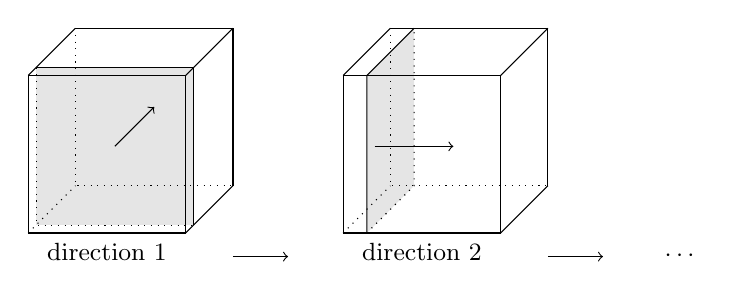
\begin{tikzpicture}
	\fill[color=gray!20] (0,0) -- (2,0) -- (2,2) -- (0,2) -- cycle;
	\draw [dotted] (0,2)  -- (0,0) -- (2,0) ;
	\draw (2,0) -- (2,2) -- (0,2) ;
	\draw (-0.1,-0.1) -- (1.9,-0.1) -- (1.9,1.9) -- (-0.1,1.9) -- cycle;
	\draw [dotted] (0.5,2.5) -- (0.5,0.5) -- (2.5,0.5);
	\draw (2.5,0.5) -- (2.5,2.5) -- (0.5,2.5);
	\draw (1.9,1.9) -- (2.5,2.5);
	\draw (-0.1,1.9)--(0.5,2.5);
	\draw (1.9,-0.1)--(2.5,0.5);
	\draw[dotted] (-0.1,-0.1)--(0.5,0.5);
	\draw[->] (1,1) -- (1.5,1.5);
	\draw(0.9,-0.1) node[below]{\small direction 1} ;
	
	\fill[color=gray!20] (4.2,-0.1) -- (4.2,1.9) -- (4.8,2.5) -- (4.8,0.5) -- cycle;
	\draw (4.2,-0.1) -- (4.2,1.9) -- (4.8,2.5);
	\draw[dotted] (4.2,-0.1) -- (4.8,0.5) -- (4.8,2.5);
	\draw (3.9,-0.1) -- (5.9,-0.1) -- (5.9,1.9) -- (3.9,1.9) -- cycle;
	\draw [dotted] (4.5,2.5) -- (4.5,0.5) -- (6.5,0.5);
	\draw (6.5,0.5) -- (6.5,2.5) -- (4.5,2.5);
	\draw (3.9,1.9) -- (4.5,2.5);
	\draw (5.9,1.9)--(6.5,2.5);
	\draw (5.9,-0.1)--(6.5,0.5);
	\draw[dotted] (3.9,-0.1)--(4.5,0.5);
	\draw[->] (4.3,1) -- (5.3,1);
	\draw(4.9,-0.1) node[below]{\small direction 2} ;
	\draw[->] (2.5,-0.4) -- (3.2,-0.4);
	\draw[->] (6.5,-0.4) -- (7.2,-0.4);
	\draw(8.2,-0.2) node[below]{\small $\cdots$} ;
	\end{tikzpicture}
	\caption{2-dimensional splitting for numerical resolution.}
	\label{fig:split2d}
\end{figure}

 


\end{document}